\section{Ejercicio 1}

En la Fig. 1 se puede observar el espectro en frecuencias de la señal de mensaje $m(t)$.

\begin{figure}[h!]
    \centering
    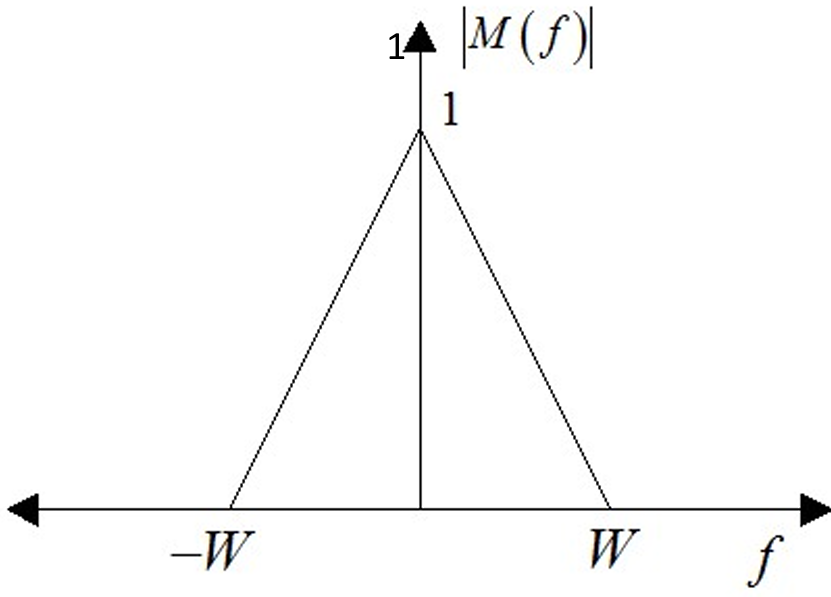
\includegraphics[width=0.7\textwidth]{imagenes/Parte_1/Actividad_1/fig1.png}
    \caption{Espectro en frecuencias de la señal de mensaje $m(t)$}
\end{figure}

El ancho de banda de la señal es de 1000 Hz, y es aplicada a un modulador producto, el cual posee una portadora $A \cos(2 \pi f t)$. La señal modulada $s(t)$ es luego aplicada a un Detector Coherente como el indicado en la Fig. 2 del Ejercicio 4.

\begin{enumerate}[label=\alph*)]
    \item Graficar el espectro obtenido en la salida del detector, para $f = 500$ Hz. Suponer la portadora del modulador producto en perfecto sincronismo con la del Detector Coherente. ¿Se recibe la señal enviada? Justifique.
    \item Proceder de manera similar al punto anterior, pero esta vez suponiendo $f = 10$ kHz.
    \item ¿Cuál es la mínima frecuencia de portadora que debería emplearse de manera tal de poder recuperar $m(t)$ a través de $s(t)$, sin distorsión?
\end{enumerate}
